%==============================================================================
\documentclass[11pt,oneside,onecolumn,letterpaper]{article}
\usepackage{times}
\usepackage[paperwidth=8.5in, paperheight=11in,
top=2.5cm, bottom=2.6cm, left=2.58cm, right=2.53cm]{geometry}
%\setlength{\textheight} {9.00in}
%\setlength{\textwidth}  {6.40in}
%\setlength{\topmargin}  {-0.50in}
%%\setlength{\headheight} {0.00in}
%%\setlength{\headsep}     {0.40in}
%\setlength{\oddsidemargin}{-0.010in}
%\setlength{\evensidemargin}{-0.00in}
%==============================================================================
%\usepackage{algorithm}
\usepackage{amssymb}
\usepackage{color,soul}
\usepackage{booktabs}
\usepackage{graphicx}
\usepackage{latexsym}
\usepackage{subfigure}
\usepackage{wrapfig}
\usepackage{amsmath}
\usepackage{amsthm}
\usepackage[hyphens]{url}
\usepackage{pifont}
\usepackage{xcolor}
\usepackage{colortbl}
\usepackage{indentfirst}
\usepackage[lined, boxed, linesnumbered]{algorithm2e}
\usepackage[square, comma, sort&compress, numbers]{natbib}

\newcounter{alg}
\newenvironment{enum-ref}{
\begin{list}%
{[\arabic{alg}]} {\usecounter{alg}
  \setlength{\leftmargin} {0.25in}
  \setlength{\labelwidth} {0.30in}
  \setlength{\rightmargin}{0.00in}
  \setlength{\topsep}     {0.00in}}
}{\end{list}}

\newenvironment{enum-number}{
\begin{list}%
{\arabic{alg})} {\usecounter{alg}
  \setlength{\leftmargin} {0.25in}
  \setlength{\labelwidth} {0.30in}
  \setlength{\rightmargin}{0.00in}
  \setlength{\topsep}     {0.00in}}
}{\end{list}}

\newenvironment{enum-nonum}{
\begin{list}%
{$\bullet$} {
  \setlength{\leftmargin} {0.25in}
  \setlength{\labelwidth} {0.30in}
  \setlength{\rightmargin}{0.00in}
  \setlength{\topsep}     {0.00in}}
}{\end{list}}

\newcommand{\ziming}[1]{%
  \begingroup
  \definecolor{hlcolor}{RGB}{20, 255, 20}\sethlcolor{hlcolor}%
  \textcolor{black}{\hl{\textit{\textbf{Ziming:} #1}}}%
  \endgroup
}

\let\chapter\section

%==============================================================================
\pagestyle{plain}
%==============================================================================

\title{Protected Automotive Remote Entry Device (PARED) \\ System Design}
\author{MITRE eCTF 2023\\Team \textbf{Cacti}\\ University at Buffalo}
\date{}



\begin{document}
%%
%=============================================================================
\normalsize


\maketitle
%\date{}

\renewcommand{\thepage}{System Design, Team Cacti, University at Buffalo--\arabic{page}}
\setcounter{page}{1} \normalsize
%
%\renewcommand{\baselinestretch}{1.2}
%\normalsize
%\vspace{0.1in}
%\centerline{\textbf{\Large }}
%\renewcommand{\baselinestretch}{1.0}
%\normalsize

\newcommand{\flagRollback}{\textsf{Rollback}\xspace}

\section{Introduction}

The following summarizes the entities in the system.
\begin{itemize}
	\item Our design will consist of four main components: host computer, car, paired fob, and unpaired fob.
	\item The host computer is a general-purpose computer used to communicate with the car and fob devices over a serial interface. These tools will be used to pair a new fob with a specific car and to instruct a paired fob to unlock a car. They can also be used to package and enable a feature for a specific car.
	\item The main purpose of the paired fob is to unlock a car. Additionally, an unpaired fob can be paired to work with a specific car.
\end{itemize}

The following summarizes the features in the system.
\begin{itemize}
	\item The owner of a car will receive pre-paired fobs that unlock their car. 
	\item The manufacturer will also produce unpaired fobs that any owner can pair with their car.
	\item If a car owner pays for an upgraded feature, then the manufacturer will send them a file to install onto an existing paired fob, which will then enable the upgraded feature on their car.
\end{itemize}

\section{Security Requirements}

This section defines the security requirements of our design.

\subsection{SR1}
\textbf{A car should only unlock and start when the user has an authentic fob that is paired with the car.}

\paragraph{How we address it:}
In our design, each car-fob-pair will have its unique RSA key pair, and only the paired fob with the correct private key can unlock and start the car.
If the fob is unpaired or paired with another car, it won't have the correct private key corresponds to the public key in the car and thus cannot unlock and start the car.

\subsection{SR2}
\textbf{Revoking an attacker's physical access to a fob should also revoke their ability to unlock the associated car.}

\paragraph{How we address it:}
When the attacker has physical access to a fob, they will not be able to pair an unpaired fob without the correct pairing PIN.
In our design, we try to minimize the possibility of an attacker hijacking the control flow and bypassing the checks before sending out the pairing info package.
We configure the MPU to set the stack as non-executable to prevent executing shellcode.
This security requirement also relates to the replay attack. Refer to the SR3 to see how we address it.

\subsection{SR3}
\textbf{Observing the communications between a fob and a car while unlocking should not allow an attacker to unlock the car in the future.}

\paragraph{How we address it:}
To prevent the attack from using the previous communications during an unlock procedure, we enforce the challenge-and-answer rule during the unlock communication.
In each unlocking procedure, the car will generate a random package as the challenge, and the paired fob has to encrypt it and send the encrypted answer back to get it verified at the car side.
In this case, the communication between a fob and a car will differ in each unlocking procedure.
Thus, the attack will not be able to perform the replay attack with previously observed communications.

\subsection{SR4}
\textbf{Having an unpaired fob should not allow an attacker to unlock a car without a corresponding paired fob and pairing PIN.}

\paragraph{How we address it:}
To prevent the PIN extraction attack, the pairing PIN will never be saved or sent in plain text.
To prevent the brute force attack on the pairing PIN, the paired fob will be in lockout for 5 seconds after each paring request with the incorrect pairing PIN.
With only a paired fob, the attacker can never trigger the sending out of the pairing info package without a correct pairing PIN.
With only the pairing PIN, the attack can never pair an unpaired fob without a paired fob since the secrets to unlock the car are stored in the paired fob.

\subsection{SR5}
\textbf{A car owner should not be able to add new features to a fob that did not get packaged by the manufacturer.}

\paragraph{How we address it:}
In our design, the feature package is signed by a private key which stores at the \textit{secrets} docker volume, and verified with a public key, which stores at the fob.
The private key will never leave the \textit{secrets} docker volume, so the attacker won't be able to use it to encrypt a feature package.
The packages that are not encrypted by the private key will not pass the public key verification on the fob device.
In other words, a valid feature package can only be packed by the manufacturer.

\subsection{SR6}
\textbf{Access to a feature packaged for one car should not allow an attacker to enable the same feature on another car.}

\paragraph{How we address it:}
In our design, if a packaged feature gets decrypted successfully on a paired fob, the fob will compare the car ID from the decrypted feature package with the one stored in the paired fob.
Thus, providing a feature package from another car will not pass the checks on the paired fob.

During the unlock, the signed feature list will be sent to the car, and this RSA key is protected during the pairing procedure.
Thus, the attacker cannot retrieve this unlock RSA key from the pairing info package to encrypt an arbitrary feature list.
They also cannot manipulate the feature list sent to the car during the unlock procedure.


\section{Security Implementations}

During the booting of the device, the MPU setting is configure to 1) set the SRAM region (\verb|0x20000000| to \verb|0x20008000|) as eXecute-Never (XN), and 2) set the code flash region (\verb|0x00008000| to \verb|0x00023800|) as read-only.

\subsection{Build PARED System}

\subsubsection{Build Environment}

This step will build the docker image from the Dockerfile. We will list all the additional packages we used besides those are in the reference design.

\subsubsection{Build Tools}

\textit{The resulting host tools will be given to the other teams in the Attack Phase.}

Our host tools are written in Python, thus this step will simply copy all the tools in to the docker container.

\subsubsection{Build Deployment}

\textit{Attackers will NEVER be given access to the Host Secrets generated in this step.}

In our design, the Host Secrets contain two parts: the Deployment Secrets and the Build Secrets, and they will be saved in the \textit{secrets} docker volume.

\begin{figure}[!htbp]
	\begin{centering}
		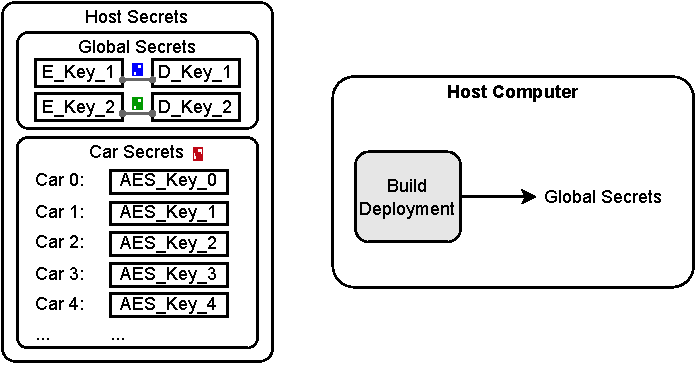
\includegraphics[width = .6\textwidth]{pic/build_depl.pdf}
		\caption{Host Secrets and Build Deployment Step}
		\label{fig:build_depl}
	\end{centering}
\end{figure}

This step will generate the Deployment Secrets, a deployment-wide secret shared across cars and fobs.
The Deployment Secrets have two pairs of asymmetric encryption (RSA) keys.
The first pair is used for encrypting the packaged feature and authenticating it.
The \verb|Feature_Priv| is used for packaging the feature and will never get loaded to any car/fob devices.
The \verb|Feature_Pub| is used to authenticate the packaged feature and will get loaded to the fob devices.
The second pair is used for encrypting and authenticating the pairing info package sent from the paired fob to the unpaired fob to prevent information leakage from the pairing info package.
The \verb|Pair_Pub| is used for encrypting the pairing info package and will be loaded to the paired fob devices.
The \verb|Pair_Priv| is used for decrypting the pairing info package and will be loaded to the unpaired fob devices.
After an unpaired fob gets paired, the saved \verb|Pair_Priv| will be erased.

We generate the Deployment Secrets randomly, to prevent the attacker from retrieving it through the source code.

\subsubsection{Build Car, Paired Fob, and Unpaired Fob}

\textit{The plaintext firmware and EEPROM files produced in these steps are not given to attackers except for the car and paired fob of Car 0 that will not contain any flags.}

\textit{These build steps may read and modify the Host Secrets.}

\begin{figure}[!htbp]
	\begin{centering}
		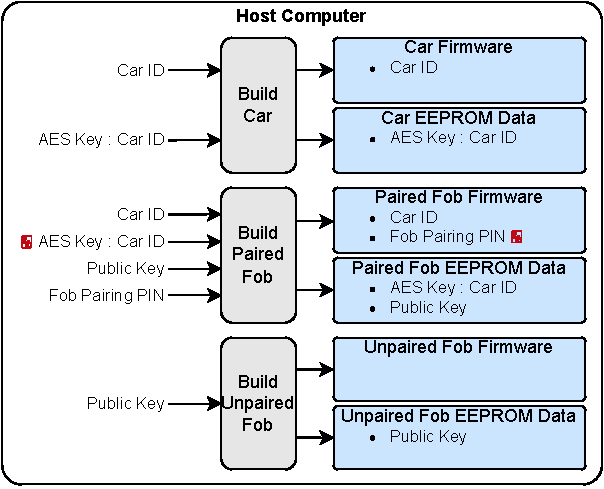
\includegraphics[width = .6\textwidth]{pic/build_step.pdf}
		\caption{Build Steps}
		\label{fig:build_step}
	\end{centering}
\end{figure}

To build the car binaries, a car ID will be supplied as a flag to the building tools. We will:
\begin{itemize}
	\item Check whether the unlock RSA key pair that corresponding to this car ID (\verb|Unlock_Priv:CarID| and \verb|Unlock_Pub:CarID|) exists in the \textit{secrets} docker volume.
	\item If it not exists, we randomly generate one, and save it into the \textit{secrets} docker volume.
	\item This \verb|Unlock_Pub:CarID| will get loaded into the car EEPROM data. The car ID will be saved in the car firmware.
\end{itemize}

To build the paired fob binaries, a car ID (corresponding to this fob) and a fob pairing PIN will be supplied as a flag to the building tools. We will:
\begin{itemize}
	\item Retrieve the private unlock RSA key which corresponding to this car ID (\verb|Unlock_Priv:CarID|) from the \textit{secrets} docker volume.
	\item Retrieve the \verb|Feature_Pub| and \verb|Pair_Pub| from the \textit{secrets} docker volume.
	\item Generate a hash for the fob pairing PIN and \verb|Pair_Pub|.
	\item Save the \verb|Unlock_Priv:CarID|, \verb|Feature_Pub|, and \verb|Pair_Pub| into the paired fob EEPROM data. Save the car ID and the hash in the paired fob firmware.
\end{itemize}

To build the unpaired fob binaries, we will:
\begin{itemize}
	\item Retrieve the \verb|Feature_Pub|, \verb|Pair_Pub| and \verb|Pair_Priv| from the \textit{secrets} docker volume.
	\item Save the the \verb|Feature_Pub|, \verb|Pair_Pub| and \verb|Pair_Priv| into the paired fob EEPROM data.
\end{itemize}

\subsection{Load Devices}

\textit{Teams will not be able to modify any part of this step.}

After building the system, the firmware and EEPROM contents are loaded onto the microcontrollers by the provided tools.

\subsection{Host Tools}

\subsubsection{Package Feature}

\textit{Attackers will be given access to the packaged feature produced in this step in many scenarios.}

\begin{figure}[!htbp]
	\begin{centering}
		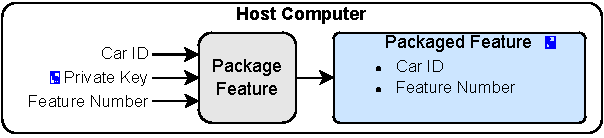
\includegraphics[width = .6\textwidth]{pic/package_feature.pdf}
		\caption{Package Feature Step}
		\label{fig:package_feature}
	\end{centering}
\end{figure}

The package feature host tool receives the car ID and the feature number as flags, and is able to read the host secrets.
\begin{itemize}
	\item Pack the the car ID, feature number and a random token together.
	\item Retrieve the \verb|Feature_Priv| from the \textit{secrets} docker volume.
	\item Sign the package using the \verb|Feature_Priv| and append the signature to the package.
\end{itemize}

The resulting packaged feature is signed by the \verb|Feature_Priv|, and this private RSA key will never be stored outside of the \textit{secrets} docker volume.

\subsubsection{Pair Fob}

\textit{This tool will not have access to Host Secrets.}

The following describes the sequence of pairing an unpaired key fob. It requires the host tool, a paired fob device, and an unpaired fob. The paired and unpaired fobs are connected to the host computer through the UART0 and also connect to each other through the UART0. The host tool takes a pairing PIN as an argument, which needs to be the same pairing PIN as previously used to pair/build the paired fob.

Protection key-points: \textbf{confidentiality of the pairing PIN; confidentiality of the pairing info package.}

\begin{figure}[!htbp]
	\begin{centering}
		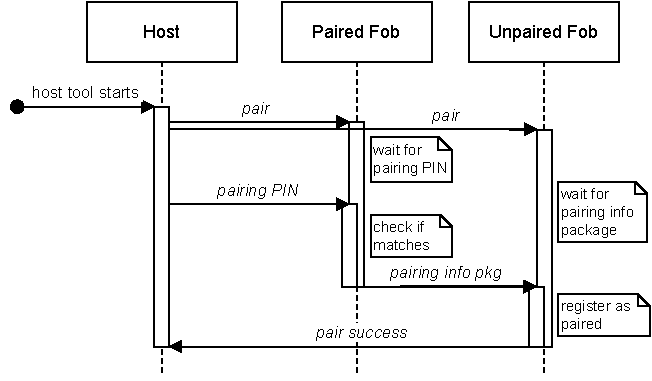
\includegraphics[width = .6\textwidth]{pic/pair.pdf}
		\caption{Pair Fob Sequence}
		\label{fig:pair}
	\end{centering}
\end{figure}

\begin{enumerate}
	\item The host tool starts the connection to both the paired and unpaired fob's UART0 for serial transaction.
	\item The host tool sends the \textit{pair} command to both the paired and unpaired fob's sockets.
	\item After the paired fob receives the \textit{pair} command, it will enter the state to waiting for receiving the pair PIN from the same UART0.
	\item After the unpaired fob receives the \textit{pair} command, it will enter the state to waiting for receiving the pairing info package from the UART1 which connects to the paired fob.
	\item The host tool sends the pairing PIN to the paired fob's UART0.
	\item The paired fob receives the pairing PIN and hashes the pairing PIN and \verb|Pair_Pub|. Then it checks the hashing result with the saved hash. If it matches, the paired fob will pack and encrypt the pairing info package with a random-generated AES key, and encrypt the AES key with the \verb|Pair_Pub|. Then it send the RSA-encrypted AES key and the AES-encrypted pairing info to the UART1. If the hash does not match, the paired fob will lockout for 5 seconds before resuming to listen to the UART messages.
	\item If the unpaired fob receives the pairing info package through the UART1 socket which connects to the paired fob, it will first decrypt AES key package with the \verb|Pair_Priv| and use the AES key to decrypt the pairing info package. Then the unpaired fob uses the info inside to register it as a paired fob.
	\item The unpaired fob (now it's paired) sends the pairing successful message to the UART0 to the host tool.
\end{enumerate}

Notes:
\begin{itemize}
	\item If the pairing PIN check in the paired fob fails, the paired fob will enter the lockout mode which blocks all the UART communication for 5 seconds. This is to prevent the brute force cracking of the pairing PIN.
	\item The pairing info package contains the car ID, the \verb|Unlock_Priv:CarID|, and the hashed pairing PIN.
	\item After the unpaired fob registers it as a paired fob, the saved \verb|Pair_Priv| will be overwritten by the \verb|Unlock_Priv:CarID|.
\end{itemize}

\subsubsection{Enable Feature}

\textit{This tool will not have access to Host Secrets.}

The following describes the sequence of enabling a feature on a paired key fob. It requires the host tool, a paired fob device, and the packaged feature file. The paired fob is connected to the host computer through the UART0.

Protection key-points: \textbf{integrity of the packaged feature.}

\begin{figure}[!htbp]
	\begin{centering}
		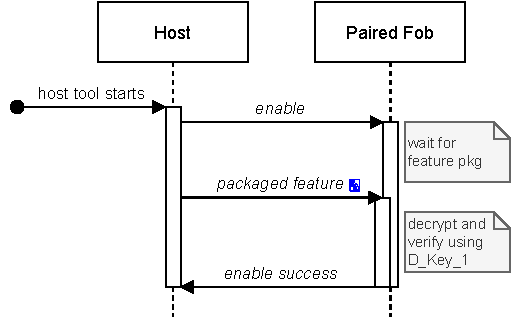
\includegraphics[width = .5\textwidth]{pic/enable.pdf}
		\caption{Enable Feature Sequence}
		\label{fig:enable}
	\end{centering}
\end{figure}

\begin{enumerate}
	\item The host tool starts the connection to the paired fob's UART0 for serial transaction.
	\item The host tool sends the \textit{enable} command to the paired fob's UART0.
	\item After the paired fob receives the \textit{enable} command, it will enter the state to waiting for receiving the packaged feature from the same UART0.
	\item The host tool reads and sends the content of the packaged feature to the paired fob's UART0.
	\item The paired fob receives and verifies the feature data with the \verb|Feature_Pub|. If 1) the car ID in data matches the saved car ID, 2) the enabled feature list is not full, and 3) this feature has not been enabled previously, the paired fob will enable this feature and save the new feature list.
	\item The paired fob sends the enable successful message to the UART0 to the host tool.
\end{enumerate}

Notes:
\begin{itemize}
	\item The paired fob uses the \verb|Feature_Pub| and the received signature to verify the received feature data.
\end{itemize}

\subsubsection{Unlock and Start Car}

\textit{This tool will not have access to Host Secrets.}

The following describes the sequence of unlocking the car with a paired fob. It requires the host tool, a paired fob device, and a car device. The car device is connected to the host computer through the UART0, and the paired fob connects to the car through the UART1. The connection between the car device and the host computer is only responsible for transmitting the messages that get printed out after the successful unlock.

Protection key-points: \textbf{authenticity of the paired fob; integrity of the feature list.}

\begin{figure}[!htbp]
	\begin{centering}
		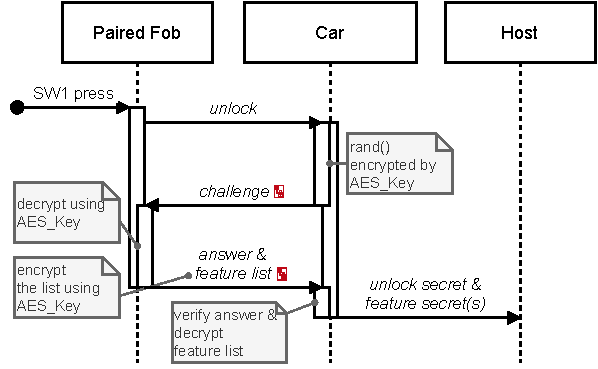
\includegraphics[width = .6\textwidth]{pic/unlock.pdf}
		\caption{Unlock Car Sequence}
		\label{fig:unlock}
	\end{centering}	
\end{figure}

\begin{enumerate}
	\item The user press the SW1 button on the paired fob.
	\item The paired fob sends the \textit{unlock} command to the UART1, and enter the state to waiting for receiving a respond from the same UART1 socket.
	\item After the car receives the \textit{unlock} command, it will generate a random value. This random value is called \textit{challenge}.
	\item The car sends the \textit{challenge} package to the the UART1, and enter the state to waiting for receiving a respond from the same UART1.
	\item The paired fob receives the \textit{challenge} package and get this random value. Then it hashes the combination of this random value and the current feature info, and sign it with the \verb|Unlock_Priv:CarID|. The resulting signature is called \textit{answer}, which will be sent to the UART1 to the car with the feature info package.
	\item The car receives the \textit{answer} and verifies it with the combination of the previous random value and the feature info using \verb|Unlock_Pub:CarID|. If the verification passes, the car will send the unlock secret and then match the feature list and send the feature secret(s) to the UART0 to the host computer.
\end{enumerate}

\end{document}
%==============================================================================
